% Template from https://www.overleaf.com/latex/templates/ieee-conference-template/grfzhhncsfqn
\documentclass[conference]{IEEEtran}
\IEEEoverridecommandlockouts
% The preceding line is only needed to identify funding in the first footnote. If that is unneeded, please comment it out.
\usepackage{cite}
\usepackage{amsmath,amssymb,amsfonts}
\usepackage{algorithmic}
\usepackage{graphicx}
\usepackage{textcomp}
\usepackage{xcolor}
\def\BibTeX{{\rm B\kern-.05em{\sc i\kern-.025em b}\kern-.08em
    T\kern-.1667em\lower.7ex\hbox{E}\kern-.125emX}}
\begin{document}

% From: https://tex.stackexchange.com/a/458208
\makeatletter
\newcommand{\linebreakand}{%
  \end{@IEEEauthorhalign}
  \hfill\mbox{}\par
  \mbox{}\hfill\begin{@IEEEauthorhalign}
}
\makeatother

\title{Vehicle-to-Vehicle (V2V) Communication Implementation\\
\thanks{University of Florida}
}

\author{
    \IEEEauthorblockN{Gunnar Fandrich}
    \IEEEauthorblockA{
        \textit{Group: Autogators} \\
        \textit{Electrical and Computer Engineering} \\
        \textit{University of Florida} \\
Gainesville, Florida \\
gunnarfandrich@ufl.edu
    }
    \and
    \IEEEauthorblockN{Mark Lai}
    \IEEEauthorblockA{
        \textit{Group: Autogators} \\
        \textit{Electrical and Computer Engineering} \\
        \textit{University of Florida} \\
Gainesville, Florida \\
marklai@ufl.edu
    }
    \and
    \IEEEauthorblockN{Rafael Hernandez-Lopez}
    \IEEEauthorblockA{
        \textit{Group: Autogators} \\
        \textit{Electrical and Computer Engineering} \\
        \textit{University of Florida} \\
Gainesville, Florida \\
rhernandezlopez1@ufl.edu
    }
    \linebreakand
    \IEEEauthorblockN{Rohan Malik}
    \IEEEauthorblockA{
        \textit{Group: Autogators} \\
        \textit{Electrical and Computer Engineering} \\
        \textit{University of Florida} \\
Gainesville, Florida \\
rmalik@ufl.edu
    }
}

\maketitle

\begin{abstract}
Vehicle-to-vehicle (V2V) allows communication between vehicles, promoting driver
awareness and potentially reducing the number of collisions. Existing V2V
implementations (cellular vehicle-to-everything, C-V2X) rely on cloud data,
whereas the implementation shown in this paper does true V2V between vehicles. A
mockup utilizing two ESP32 with a time-of-flight (ToF) sensor and accelerometer
communicate using UDP to deliver a proof-of-concept for V2V that can be used as
a base for V2V.
\end{abstract}

\begin{IEEEkeywords}
V2V, vehicles, driver, awareness, C, ESP32, WiFi, UDP, UDP Broadcast
\end{IEEEkeywords}

\section{Introduction}
\subsection{Problem Statement}
As society moves towards utilizing more autonomous driving systems, vehicles can
act as a network to promote efficient and safe driving. This network is referred
to as vehicle-to-vehicle (V2V). Automotive vehicles should communicate with each
other through V2V to increase driver awareness and reduce the number of
collisions \cite{nhtsa_v2v}. A simple mockup of a V2V system should illustrate the
safety increase provided by V2V communication.

\subsection{Background and Related Works}
The current state of V2V is nonexistent. The closest thing on the market to V2V
is the 2023 Safety Cloud for Chrysler Vehicles, which is implemented through a
cellular network to create C-V2X (cellular vehicle-to-everything)
\cite{stone_2023, haas}.  While this is fairly close to V2V, passing through a
cloud does not exhibit true V2V. Ideally the cars would communicate directly to
each other, which is what is covered by the implementation discussed in this
paper. Additionally, Stellantis announced vehicle-to-grid (V2G) testing in 2019
\cite{media.stellantis_2020}.

In 1999, the FCC designated a 75 MHz spectrum in the 5.9 GHz band for dedicated
short-range communications (DSRC) \cite{hawkins_2022}. Unfortunately, this band was
reallocated in 2020 for unlicensed WiFi \cite{hawkins_2022} use due to the
failure of automobile makers to release V2X production cars. Due to the removal
of this band, we chose UDP over WiFi as an acceptable simplified protocol for
V2V. Ideally, UDP would be replaced with another protocol built on top of UDP --
or similar protocol -- specifically for V2V and operate on an FCC-designated
band for V2V.

V2V will be illustrated using an ESP32 paired with time-of-flight (ToF) sensor
and accelerometer. Each ESP32 represents a simplified car, and communicate with
each other using WiFi. UDP Broadcast was chosen as the communication protocol.

In recent years, newer vehicles have been produced with various driver warning systems.
One such driver warning system is lane departure warning. Lane departure warning has been
observed to reduce single-vehicle, side-swipe, and head-on crash severity by 11 percent
and the severity of crash injury by 21 percent \cite{iihs_bsd}. 

\section{V2V implementation}
This section covers our V2V implementation, the features and the mockup.

\subsection{Features}
The two vehicles are represented by two ESP32s. They each have a ToF sensor and
an accelerometer. The ToF sensor is used to identify whether there is another
``vehicle'' in front of the ESP32 and the accelerometer is used to know whether
the other ``vehicle'' is moving. On a real vehicle, the CAN bus can be used to
monitor and send each vehicle's velocity -- and other information as needed,
such as GPS for locating where the incoming UDP packet is coming from -- in the
UDP packet. The current UDP packet we are sending has an ID for the vehicle, the
ToF distance, and the accelerometer measurement. On the other vehicle, this
information is used to alert the driver via some LEDs. This UDP packet was standardized
between vehicles using a defined C struct to contain the relevant information.

\subsection{Hardware}
The mockup can be found on Fig.~\ref{mockup}. Each breadboard has an ESP32, a
power supply, a ToF sensor, and two LEDs. Each could have an accelerometer, but
only one ``vehicle'' had an accelerometer during testing.

\begin{figure}[htbp]
\centerline{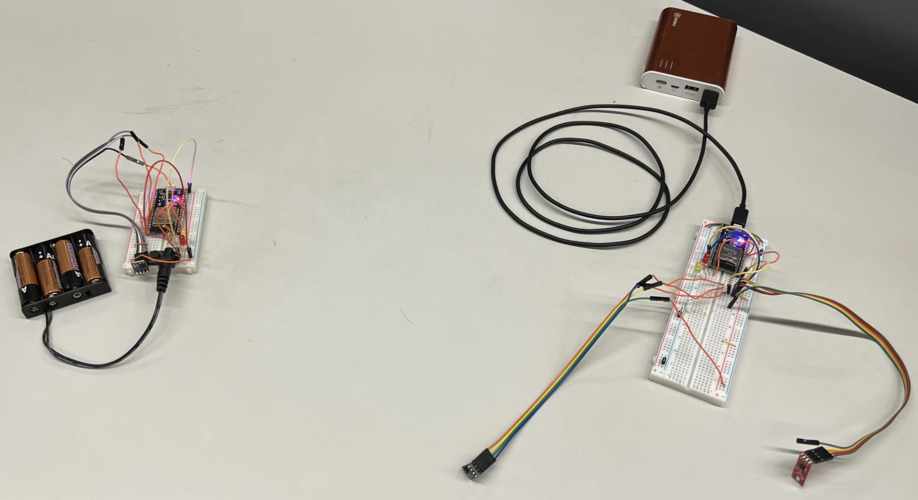
\includegraphics[width=\linewidth]{pics/two_boards.jpg}}
\caption{The mockup used to test V2V, ESP32s are ``vehicles''.}
\label{mockup}
\end{figure}

Close-ups of each ``vehicle'' can be found in Fig.~\ref{vehicle_bp} and
Fig.~\ref{vehicle_up}. The assembled ``vehicles'' can be found in
Fig.~\ref{bp_outside} and Fig.~\ref{up_outside}. They are named ``vehicle'' B
and U, respectively, from now on. B for battery pack and U for USB battery pack.

\begin{figure}[htbp]
\centerline{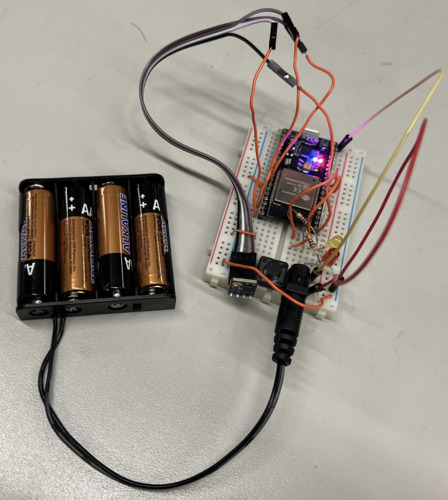
\includegraphics[width=\linewidth]{pics/bp_internals.jpg}}
\caption{One of the ``vehicles'', vehicle B, used to test our V2V implementation.}
\label{vehicle_bp}
\end{figure}

\begin{figure}[htbp]
\centerline{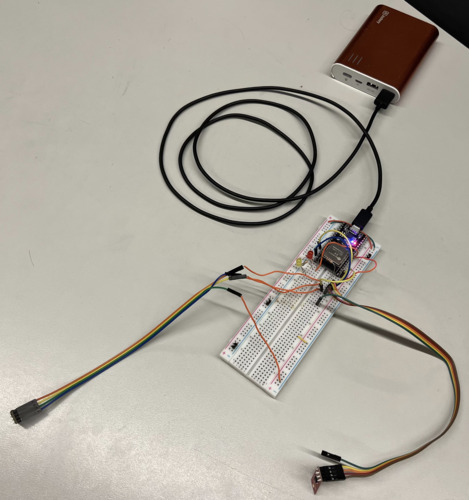
\includegraphics[width=\linewidth]{pics/up_internals.jpg}}
\caption{Another ``vehicles'', vehicle U, used to test our V2V implementation.}
\label{vehicle_up}
\end{figure}

\begin{figure}[htbp]
\centerline{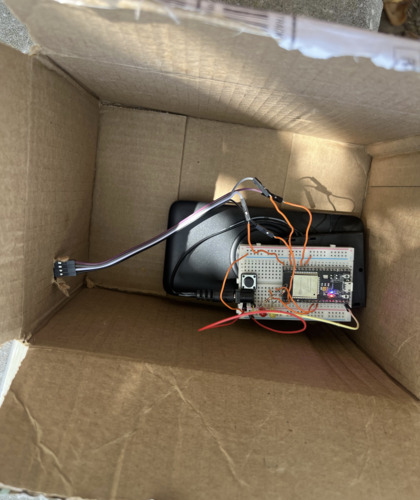
\includegraphics[width=\linewidth]{pics/bp_vehicle.jpg}}
\centerline{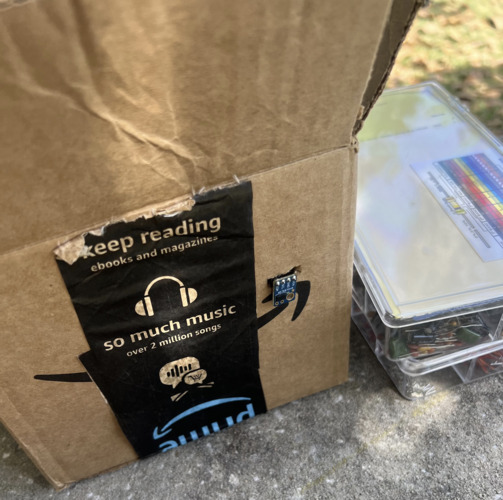
\includegraphics[width=\linewidth]{pics/bp_vehicle_outside.jpg}}
\caption{Assembled ``vehicle'', vehicle B, in our testing environment.}
\label{bp_outside}
\end{figure}

\begin{figure}[htbp]
\centerline{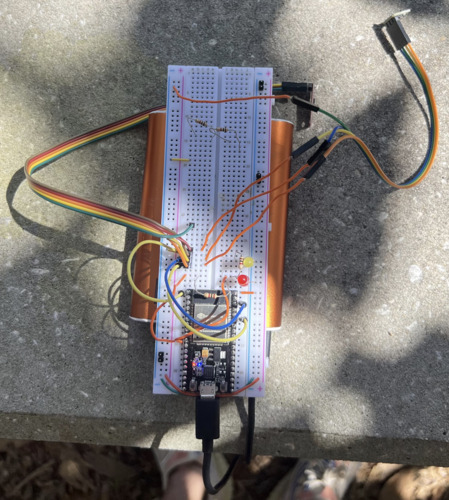
\includegraphics[width=\linewidth]{pics/up_vehicle_outside.jpg}}
\caption{Another assembled ``vehicle'', vehicle U, in our testing environment.}
\label{up_outside}
\end{figure}

The driver has two LEDs available in this implementation: a yellow ``caution''
LED, and a red ``warning'' LED. The yellow LED turns on when there is a nearby vehicle
(less than 100mm for this experiment) exchanging UDP packets with the driver's vehicle.
The red LED turns on in cases where the driver should be more cautious. To simulate this,
the red warning LED was turned on in the case that a caution message has been recieved, 
the ToF sensor has measured a distance less than or equal to 50mm, and the accelerometer
observes a negative acceleration.

Two other lights, intended for debugging, were also incorporated into the design. The blue
LED onboard the ESP32 was employed to indicate a successful boot and successful WiFi
connection between the two ESP32s. The red LED oneboard the ESP32 was utilized to 
monitor the power supply and to ensure the ESP32 was powered on.

Throughout the project's development, several hardware issues were encountered.
One of the issues was the original set of Time-of-Flight sensors not working.
This delayed the project and prompted the need for new Time-of-Flight sensors.
Fortunately, this issue was resolved quickly by ordering a new set. The new set
did not work perfectly, but this was likely due to the quality of the components.
There were intermittent disconnect issues or sporadic readings, but generally
the sensors worked and fulfilled their role in this project. Another issue encountered
during testing was power supply issues. Originally, two mobile phone battery banks were
to be used to power each ESP32, but the minimal current draw of the ESP32 caused one
of the battery banks to switch off. This battery had to be substituted for a
battery consisting of four AA batteries in series. This battery provided 6V, and the
internal power regulator of the ESP32 was able to step the voltage down to the system's
5V requirement.

\section{Results}
The two vehicles were able to be powered independently and in a portable nature.
The platoon leader vehicle hosted a WiFi access point, which the subsequent vehicle
connected to. ToF data, vehicle status, and accelerometer data was sent between each
vehicle and proccessed accordingly.

The two ``vehicles'' communicate over UDP with each other. See Fig.~\ref{term1}
to see the ``vehicle'' sending a UDP packet, and Fig.~\ref{term2} to see the
other ``vehicle'' receive the UDP packet.

\begin{figure}[htbp]
\centerline{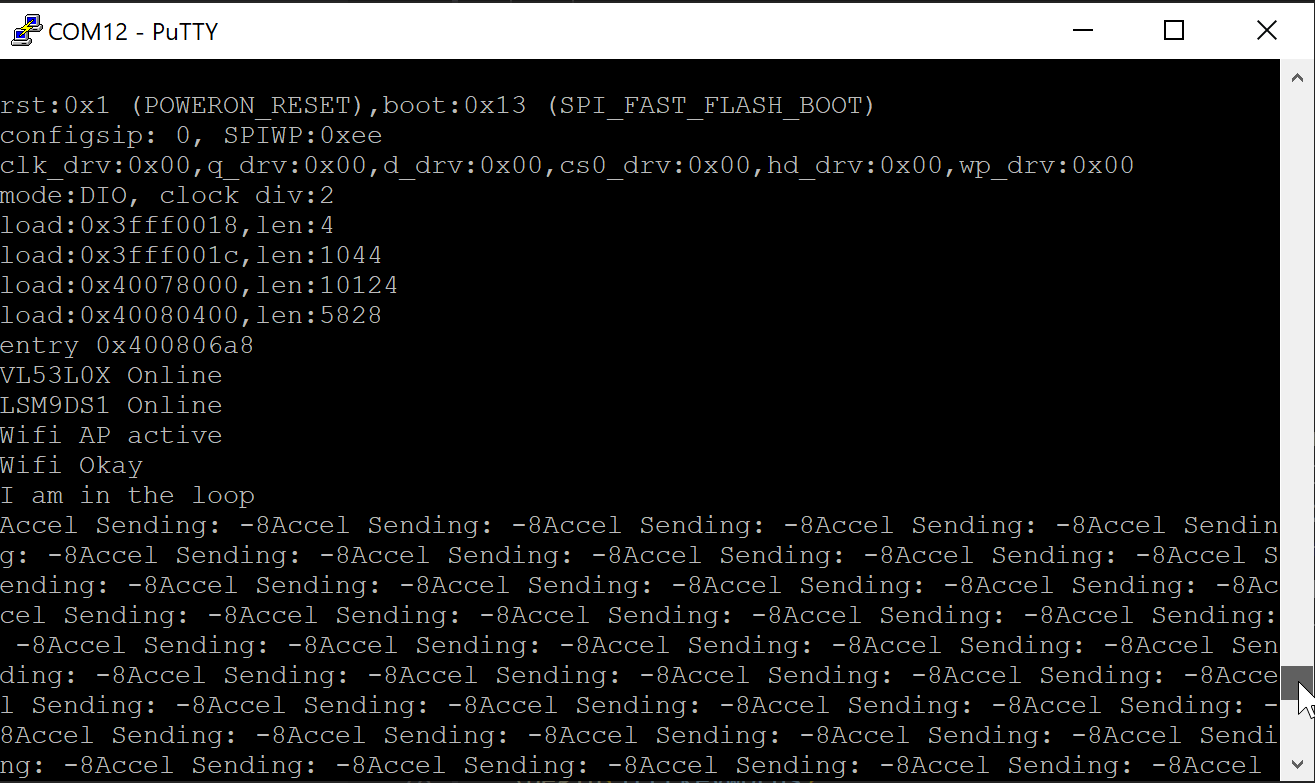
\includegraphics[width=\linewidth]{pics/term1.png}}
\caption{One ``vehicle'' is sending a message through UDP.}
\label{term1}
\end{figure}

\begin{figure}[htbp]
\centerline{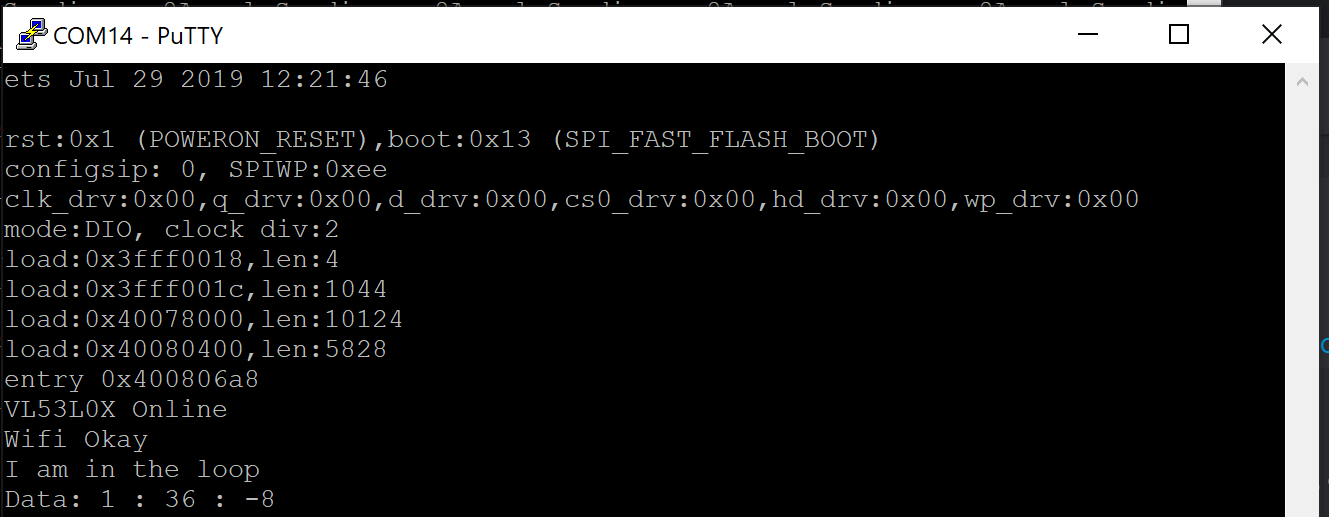
\includegraphics[width=\linewidth]{pics/term2.png}}
\caption{The other ``vehicle'' is receiving a message through UDP.}
\label{term2}
\end{figure}

\section{Security}
Our implementation of V2V has room to improve. A V2V implementation usable on
the market would address a few security concerns.

\subsection{Packet Security}
As our UDP packets are being broadcasted to everyone in the nearby vecinity, an
attacker only needs to be located near the network to be considered a ``car''.
This means that anyone could send fake messages or tamper with existing packets.
This leaves room for improvement in terms of admitting ``cars'' on the network,
and properly identifying nodes on the network as ``car'', ``adversary'', or
``miscellaneuos'' nodes.

Attackers on the network could potentially leverage this limitation to inhibit
the flow of traffic by broadcasting that there is some blockade ahead (ToF
sensor data shows car ahead, accelerometer data shows there is no/little
movement). Attackers could also target individual vehicles with a similar idea.
They could send false packets to make the victim vehicle think it has to brake
suddenly, potentially crashing with vehicles behind them or causing them to
brake too fast. If the victim is carrying a heavy load, such as a large trailer,
braking too fast can compromise the stability of their vehicle and potentially
swerve out of control or unlatch their trailer.

\subsection{Network Security}
A member of the ad-hoc network may be either callibrated to send too many
packets or is an attacker. In a case where the packet traffic is too heavy, a
denial of service attack (DoS) may occur. This should be addressed as well
before V2V is accepted by car manufacturers.

As the network is completely open to new ``cars'', attackers may be able to
probe the network for more vulnerabilities than those discussed. For example,
perhaps some UDP misconfiguration could be leveraged to forward UDP packet
contents to a CAN bus, or similar idea.

\section{Conclusion}
In this experiment, a V2V network was created using two ESP32 with ToF and
accelerometer as a proof-of-concept/base on which car manufacturers may be able
to improve and develop on.

While the protocol and protocol security demonstrated in this experiment are to
be improved, two ``vehicles'' successfully communicated and alerted a driver
of a possible hazard. Going forward, the protocol can be improved upon and 
secured to reduce the risk of false messages from adversary cars. In addition, 
a high-bandwidth band can be selected similar to the 5.9 GHz band previously
set aside by the FCC for solely V2X communications. Doing so ensures quick
short-range communication, with minimal band crowding.


%\clearpage
\bibliographystyle{IEEEtran}
\bibliography{bibs}

\end{document}

